\chapter{Implementation}
\label{implementation}
In diesem Kapitel wird die Implementation des Projekts beschrieben. Auf Basis der beschriebenen Konzeption wird im Anschluss die Implementation erfolgen. 
\section{Nachrichtenstruktur}
Da die Implementation auf einer nachrichtenbasierten Kommunikation basieren wird, ist der Entwurf eigener Nachrichtenstrukturen notwendig. Die Nachrichtenstrukturen übertragen stellen die zwischen dem Master und den Workern bereit. Konkret handelt es sich bei der gewählten Architektur nach \citep{tanenbaum} um eine \emph{Message-Queue-Architektur}. \\
Zur Strukturierung fiel die Wahl auf das Nachrichtenaustauschformat \enquote{JavaScript Object Notation} oder kurz \emph{JSON}, da dieses Format sehr leichtgewichtig und vollständig anpassbar ist. \\
Als Kommunikationsplattform wird ein Node-Server benutzt, da dieser für den vorgesehenen Bereich schnell einsetzbar und mit dem JSON-Format kompatibel ist. Der Node-Server ist für die Verteilung der Nachrichten zwischen den Rechnern des verteilten Systems verantwortlich. \\

Nachfolgend werden die entwickelten Nachrichtenstrukturen und deren Inhalt beschrieben. Zum besseren Verständnis werden die Nachrichten in die Senderichtungen zum Worker oder zum Master strukturiert. \\
Auf programmatischer Ebene wird zudem zwischen \emph{Basic Messages} und \emph{Extended Messages} unterschieden. Basic Messages beinhalten den Status des sendenden Rechners und maximal einen weiteren Wert, während Extended Messages neben dem Status mehrere Werte beinhalten. Durch diese Strukturierung ist ein effizienteres Messageparsing möglich. 

\subsection{Nachrichten vom Master an Worker}
Hier werden die Strukturen beschrieben, welche vom steuernden Rechner (Master) zu einem der Worker gesendet werden.\\

\texttt{SetupAndConfig}
\begin{lstlisting}[basicstyle=\ttfamily,numbers=left,numberstyle=\footnotesize\ttfamily,backgroundcolor=\color{sourcegray}]
{
  "status" : "setupConfig",
  "value" : {
    "algorithm" : "#HASH_ID",
    "target" : "#TARGET_HASH", 
    "worker_id" : "#WORKER_ID"
  }
}
\end{lstlisting}
Ein im Cluster neu hinzugefügter Worker erhält seine Konfigurationsparameter, damit dieser als Worker im verteilten System genutzt werden kann. 
Der Wert \textbf{algorithm} übergibt die ID des Hash-Algorithmus, welcher in der aktuellen Passwortberechnung benutzt wird. \textbf{Target} übermittelt den Hash des Zielpasswortes. Anhand des Hashes kann ein Worker bestimmen, ob das Zielpasswort berechnet wurde. Die \textbf{workerID} ist eine vom Master vergebene, fortlaufende Nummer und dient der Identifizierung der Worker.\\

\texttt{getWork}
\begin{lstlisting}[basicstyle=\ttfamily,numbers=left,numberstyle=\footnotesize\ttfamily,backgroundcolor=\color{sourcegray}]
{
  "status" : "newWorkBlog",
  "value" : {
    "worker_id" : "#WORKER_ID"
    "hashes" : ["#NEW_HASHES"]
  }
}\end{lstlisting}
Diese Nachricht übermittelt dem Worker eine Anzahl neuer Passwörter, von denen dieser die Hashes berechnen wird.\\
 %TODO Beschreibung fertigstellen.

\texttt{stillAlive}
\begin{lstlisting}[basicstyle=\ttfamily,numbers=left,numberstyle=\footnotesize\ttfamily,backgroundcolor=\color{sourcegray}]
{
  "status" : "stillAlive",
  "value" : ""
}
\end{lstlisting}
Mit Hilfe dieser Nachricht fragt der Master an, ob die angesprochenen Worker noch verfügbar sind. Wenn diese nicht antworten, werden sie der Liste der verfügbaren Worker (Worker Queue) entfernt. 


\subsection{Nachrichten vom Worker an den Master}
Folgende Nachrichten werden von den Workern an die Master gesendet. \\

\texttt{newClientRegistration}
\begin{lstlisting}[basicstyle=\ttfamily,numbers=left,numberstyle=\footnotesize\ttfamily,backgroundcolor=\color{sourcegray}]
{
  "status" : "newClientRegistration",
  "worker" : "#WORKER_ID"
}
\end{lstlisting}
Der Worker beantragt eine ID, um sich im Cluster identifizieren zu können.\\

\texttt{hitTargetHash}
\begin{lstlisting}[basicstyle=\ttfamily,numbers=left,numberstyle=\footnotesize\ttfamily,backgroundcolor=\color{sourcegray}]
{
  "status" : "hitTargetHash",
  "value" : {
    "hash" : "#HASH_VALUE",
    "password" : "#PASSWORD"
    "time_needed" : "#TIME"
    "worker_id" : "#WORKER_ID"
  }
}\end{lstlisting}
Diese Nachricht wird vom Worker versendet, wenn der berechnete Hash dem Zielhash entspricht und somit das Passwort berechnet wurde. Es werden der berechnete Hash und das zugehörige Passwort übertragen. Zudem wird die Zeit, die der Worker für die Berechnung in Anspruch genommen hat, übertragen. Die Zeit kann für spätere Erweiterungen des Projekts genutzt werden, beispielsweise zum Vergleich verschiedener Hash-Algorithmen. Allerdings gilt es zu beachten, dass sich die Zeit nur auf einen Worker bezieht. Eine globale Betrachtung der Berechnungszeit kann damit ungenau sein. \\

\texttt{finishedWork}
\begin{lstlisting}[basicstyle=\ttfamily,numbers=left,numberstyle=\footnotesize\ttfamily,backgroundcolor=\color{sourcegray}]
{
  "status" : "finishedWork",
  "value" : "#WORKER_ID"
}
\end{lstlisting}
Mit dieser Nachricht teilt der Worker mit, dass alle möglichen Passworte des aktuellen Arbeitspakets berechnet worden sind. Falls bei der Berechnung der Zielhash bzw. das Zielpasswort berechnet worden ist, wird zusätzlich die Nachricht \enquote{finishedWork} versandt. Ist das Zielpasswort noch nicht ermittelt worden, erhält der Worker ein neues Arbeitspaket, da der Master nach Erhalt der Nachricht \enquote{finished work} den Worker in den \emph{idle}-Zustand versetzt. \\

\texttt{HashesPerTime}
\begin{lstlisting}[basicstyle=\ttfamily,numbers=left,numberstyle=\footnotesize\ttfamily,backgroundcolor=\color{sourcegray}]
{
  "status" : "hashesPerTime"
  "value" : {
    "worker_id" : "#WORKER_ID"
    "hash_count" : "#NUMBER_COMPUTED_HASHES"
    "time_needed" : "#TIME"
  }
}
\end{lstlisting}
Zum Auswerten der ausgeführten Tätigkeiten übermittelt der Worker zur Identifikation seine ID und zur statistischen Auswertung sowohl die Anzahl der berechneten Hashes, als auch die zu dieser Berechnung benötigten Zeit. \\

\texttt{replyAlive}
\begin{lstlisting}[basicstyle=\ttfamily,numbers=left,numberstyle=\footnotesize\ttfamily,backgroundcolor=\color{sourcegray}]
{
  "status" : "alive",
  "value" : "#WORKER_ID"
}
\end{lstlisting}
Der Worker meldet mit dieser Nachricht, dass er dem verteilten System weiterhin zur Verfügung steht. Zur Identifikation antwortet der Worker auf die Nachricht 
\emph{stillAlive} mit seiner Worker-ID. Erfolgt auf die genannte Anfrage keine Antwort, dann entfernt der Master den nicht antwortenden Worker aus dem Array verfügbarer Worke.\\

Um Rückschlüsse auf die Geschwindigkeit verschiedener Hash-Algorithmen schließen zu können, kann bei Start der Applikation zwischen verschiedenen Hash-Algorithmen gewählt werden. Zur Auswahl stehen die Hash-Algorithmen \emph{MD5}, \emph{SHA 128} sowie \emph{SHA 256}. Die Geschwindigkeitsunterschiede beruhen primär auf der unterschiedlichen Schlüssellänge der jeweiligen Algorithmen.

\section{Benutzeroberfläche}
Nachfolgend wird die Benutzeroberfläche sowie die Interaktion mit dem verteilten System beschrieben. Da primär die Funktionalität der Anwendung im Fokus des Projekts steht, besteht die Benutzeroberfläche aus nur wenigen Interaktionselementen. \\
Die Anwendung wird auf allen Rechnern gestartet, die zum verteilten System zusammengefasst werden müssen. Je nachdem, ob der Rechner als Master oder Worker verwendet werden soll, unterscheidet sich die weitere Interaktion. Die unterschiedlichen Interaktionsmöglichkeiten werden in den folgenden Abschnitten beschrieben. 

\subsection{Master}
Durch Aktivierung des Feldes \enquote{this Mac} im Bereich \emph{Communication Manager} delegiert man den aktuellen Rechner als Master des verteilten Systems. Es gilt zu beachten, dass nur ein Master im verteilten System bestimmt wird. Nachdem diese Option gewählt wurde, wird im Feld \emph{Server Adress} die Adresse des aktuellen Rechners angezeigt. Diese Adresse wird den Workern mitgeteilt (siehe Abschnitt \ref{WorkerGUI}). Auf Abbildung \ref{fig:WindowMaster} lautet die Adresse beispielsweise \emph{127.0.0.1}, da auf dem Rechner kein Domain-Name hinterlegt worden ist. \\
\begin{figure}[!ht]
	\centering
		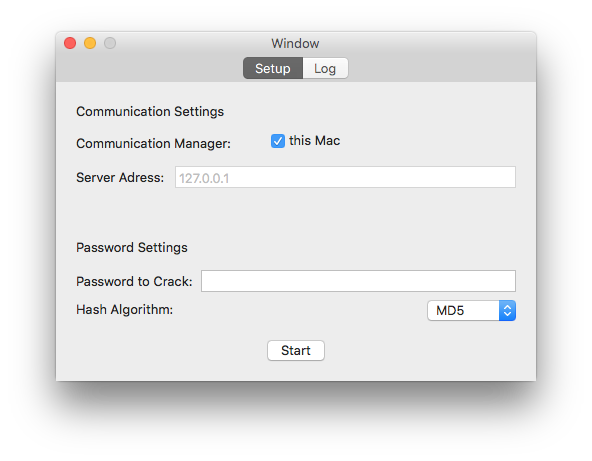
\includegraphics[natwidth=1200pt, natheight=349pt, width=0.6\textwidth]{images/WindowMaster.png}
		\caption{Benutzeroberfläche der implementierten Anwendung als Master der verteilten Anwendung}
	\label{fig:WindowMaster}
\end{figure}
Nach der Konfiguration als Master wird das Passwort festgelegt, welches entschlüsselt werden soll. Dazu wird im Feld \emph{Password to Crack} das gewünschte Passwort eingetragen werden. Abschließend kann der Hash-Algorithmus ausgewählt werden, mit dem die Hashes erzeugt werden. Die Vorgehensweise zur Entschlüsselung ändert sich dadurch nicht, die Option zur Wahl verschiedener Hash-Algorithmen dient primär zur Messung von Geschwindigkeitsunterschieden. \\

Nach Aktivierung des Start-Buttons steht der Master dem verteilten System zur Verfügung.   


\subsection{Worker}
\label{WorkerGUI}
Nachdem ein Master festgelegt wurde, können beliebig viele Rechner als Worker benutzt werden. Die Rechner müssen sich lediglich im gleichen Netz befinden. \\
Standardmäßig ist die Anwendung nach dem Start als Worker konfiguriert. Dies ist beispielsweise daran zu erkennen, dass die Möglichkeiten zum Eintragen eines Passwortes oder die Auswahl eines Hash-Algorithmus deaktiviert sind (zu erkennen auf Abbildung \ref{fig:WindowWorker}). \\
\begin{figure}[!ht]
	\centering
		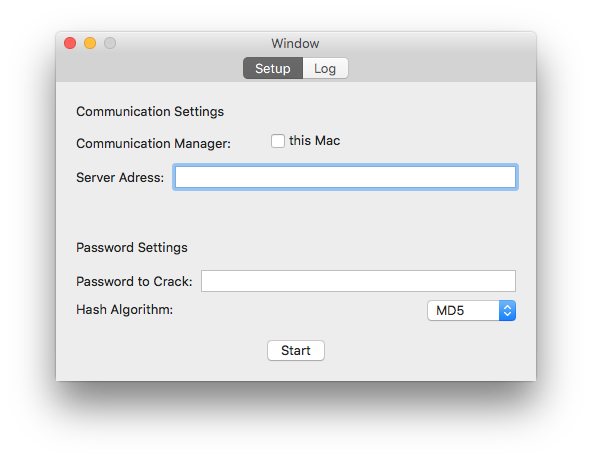
\includegraphics[natwidth=1200pt, natheight=349pt, width=0.6\textwidth]{images/WindowWorker.png}
		\caption{Benutzeroberfläche der implementierten Anwendung als Worker der verteilten Anwendung}
	\label{fig:WindowWorker}
\end{figure}
Damit der Worker mit der Berechnung beginnen kann, muss diesem die Adresse des Masters mitgeteilt werden. Diese kann aus der Anwendung des Masters entnommen werden. Im aktuellen Beispiel würde die Adresse \emph{127.0.0.1}, entnommen aus Abbildung \ref{fig:WindowMaster}, eingetragen werden.\\
Nach der Eintragung der Adresse des Masters kann die Passwortberechnung durch Betätigung des \emph{Start}-Buttons gestartet werden. 



\subsection{Auswertung des Angriffs}
Nach dem Start des Angriffs sind mehrere Beobachtungsmöglichkeiten gegeben. Die erste Möglichkeit ist das Beobachten des Logs. Dieses ist erreichbar, indem das Feld \emph{Log} ausgewählt wird.\\
Das Log stellt Informationen zu verschiedenen Ereignissen bereit. Im aktuellen Beispiel kann aus Abbildung \ref{fig:logView} entnommen werden, dass die Anwendung gestartet und der MD5-Hash-Algorithmus gewählt wurde. Zudem wird der Hash des eingegebenen Passwortes angegeben. Die Information \enquote{showing ChartView} bedeutet, dass die grafische Auswertung des Angriffs aufgerufen wurde.

\begin{figure}[!ht]
	\centering
		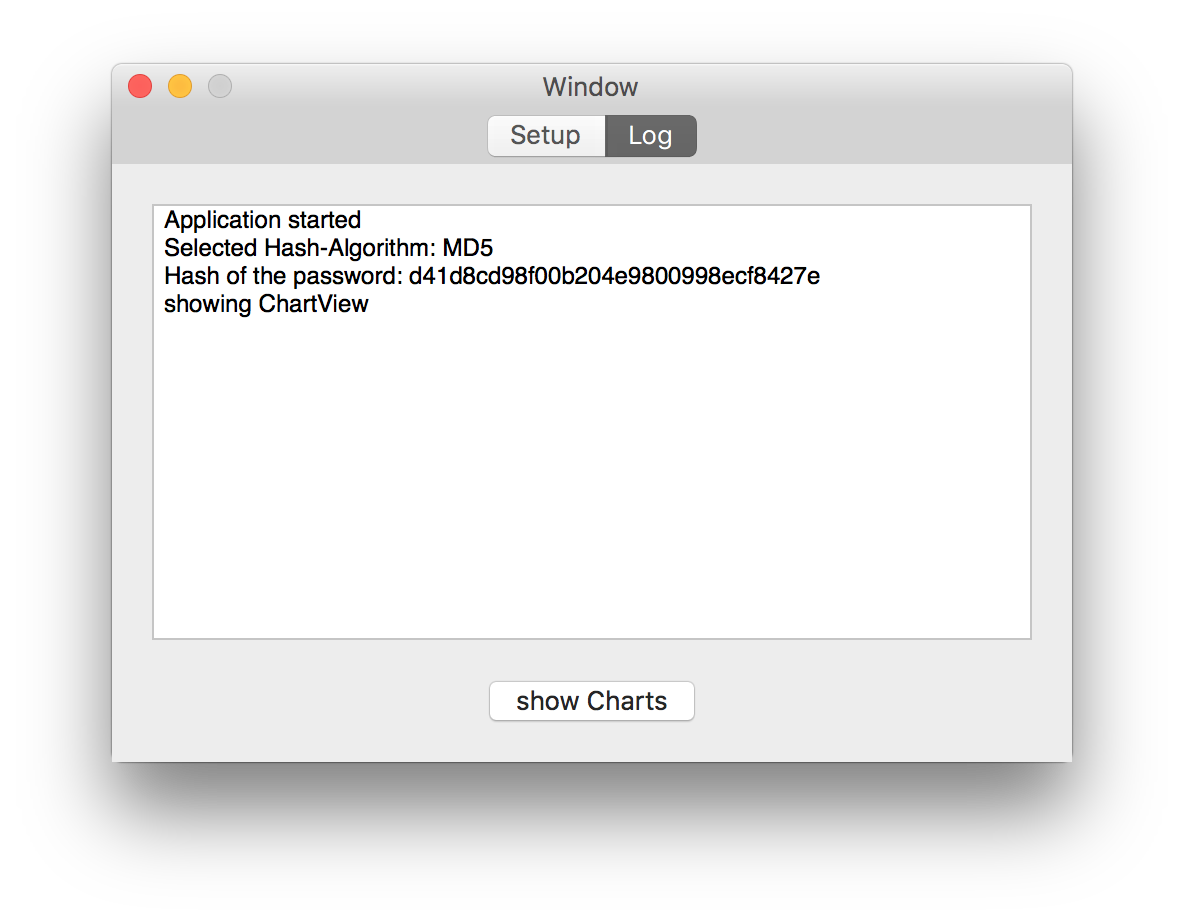
\includegraphics[natwidth=1200pt, natheight=349pt, width=0.6\textwidth]{images/logView.png}
		\caption{Log-Ansicht nach dem Start des BruteForce-Angriffs}
	\label{fig:logView}
\end{figure}

\begin{figure}[!ht]
	\centering
		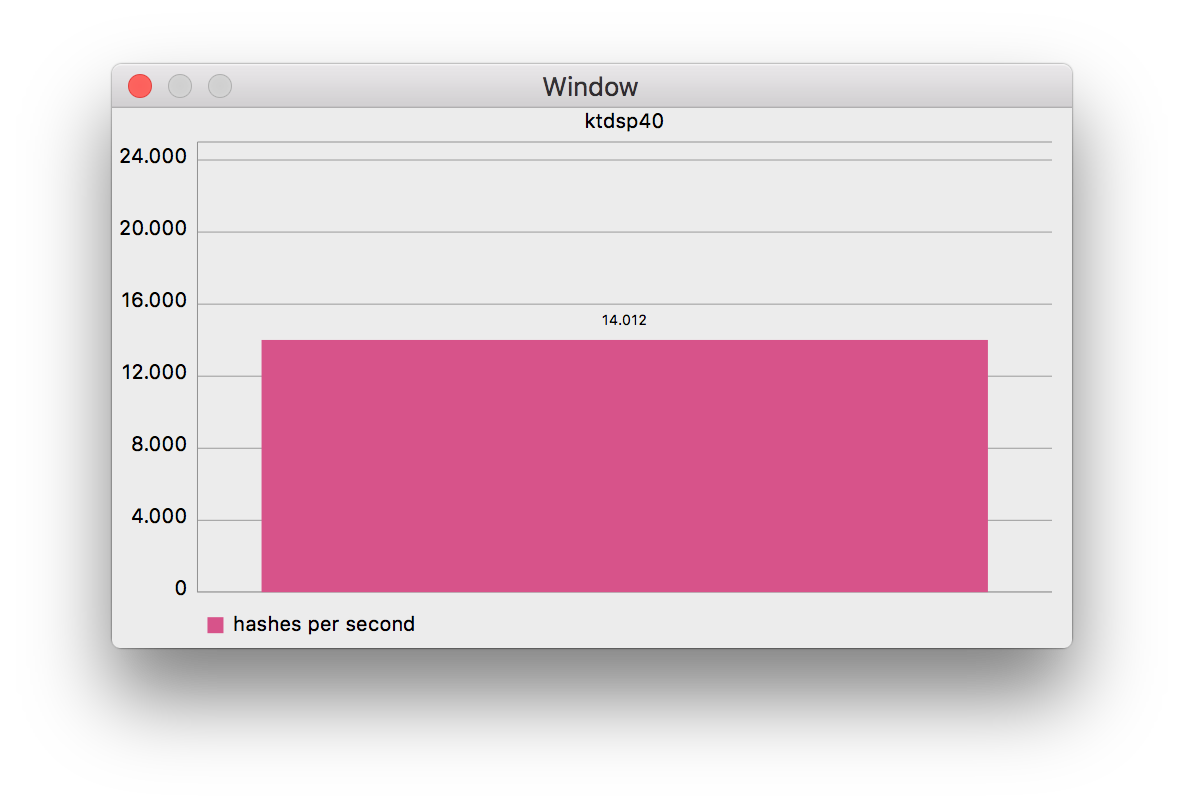
\includegraphics[natwidth=1200pt, natheight=349pt, width=0.6\textwidth]{images/chartView.png}
		\caption{Grafische Darstellung der Quantität an erzeugten Hashes pro Sekunde}
	\label{fig:chartView}
\end{figure}

Die grafische Auswertung des Angriffs ist auf Abbildung \ref{fig:chartView} dargestellt. Die Tabelle stellt in Echtzeit Informationen darüber bereit, wieviele Hashes pro Sekunde durch die jeweiligen Worker erzeugt werden. Auf Grafik \ref{fig:chartView} berechnet aktuell ein Worker 14.012 Hashes pro Sekunde. Die Diagramme zeigen den aktuellen Status der jeweiligen Worker an. Das bedeutet, dass bei Hinzufügen weiterer Worker zum System analog dazu weitere Diagramme angezeigt werden würden. 
